\section{Installare IntelliJ}
    Per svolgere gli esercizi di laboratorio, le simulazioni e l'esame userete \textbf{IntelliJ IDEA Ultimate}, non è una scelta, perciò è utile che lo usiate anche 
    quando vi esercitate a casa, inoltre imparare le varie shortcuts da tastiera vi aiuterà molto durante l'esame, sopratutto quando dovrete fare dei refactors facendovi 
    risparmiare tempo prezioso.
    Il software è normalmente a pagamento ma gli studenti hanno diritto a una licenza gratuita annuale per tutti i prodotti JetBrains, il primo step è quindi ottenere la 
    certificazione di studente.
    \subsection{Registrarsi come studente}
        È possibile registrarsi in due modi, il primo consiste nell'usare l'indirizzo email di istituto ed è quello preferibile, mentre il secondo consiste nell'inviare il certificato
        di iscrizione in inglese.
        \begin{warningbox}
            Il secondo metodo è più lungo, richiede circa una settimana perché il certificato deve essere verificato da un essere umano, ma è talvolta necessario, nel caso 
            in cui il vostro indirizzo email non venga riconosciuto.
        \end{warningbox}
        Il mio consiglio è quello di provare a registrarvi con la mail e nel caso non venisse accettata, procedere con l'invio del certificato. Indipendentemente dal metodo scelto 
        recatevi al seguente link \url{https://www.jetbrains.com/shop/eform/students}
        
        \subsubsection{Email di istituto}
            Compilate il form, prestando attenzione ad inserire l'indirizzo email nel formato 
            \textbf{nome.cognome@studenti.unitn.it}.
            \begin{figure}[H]
                \centering
                \graphicspath{{src/capitoli/04/img/}}
                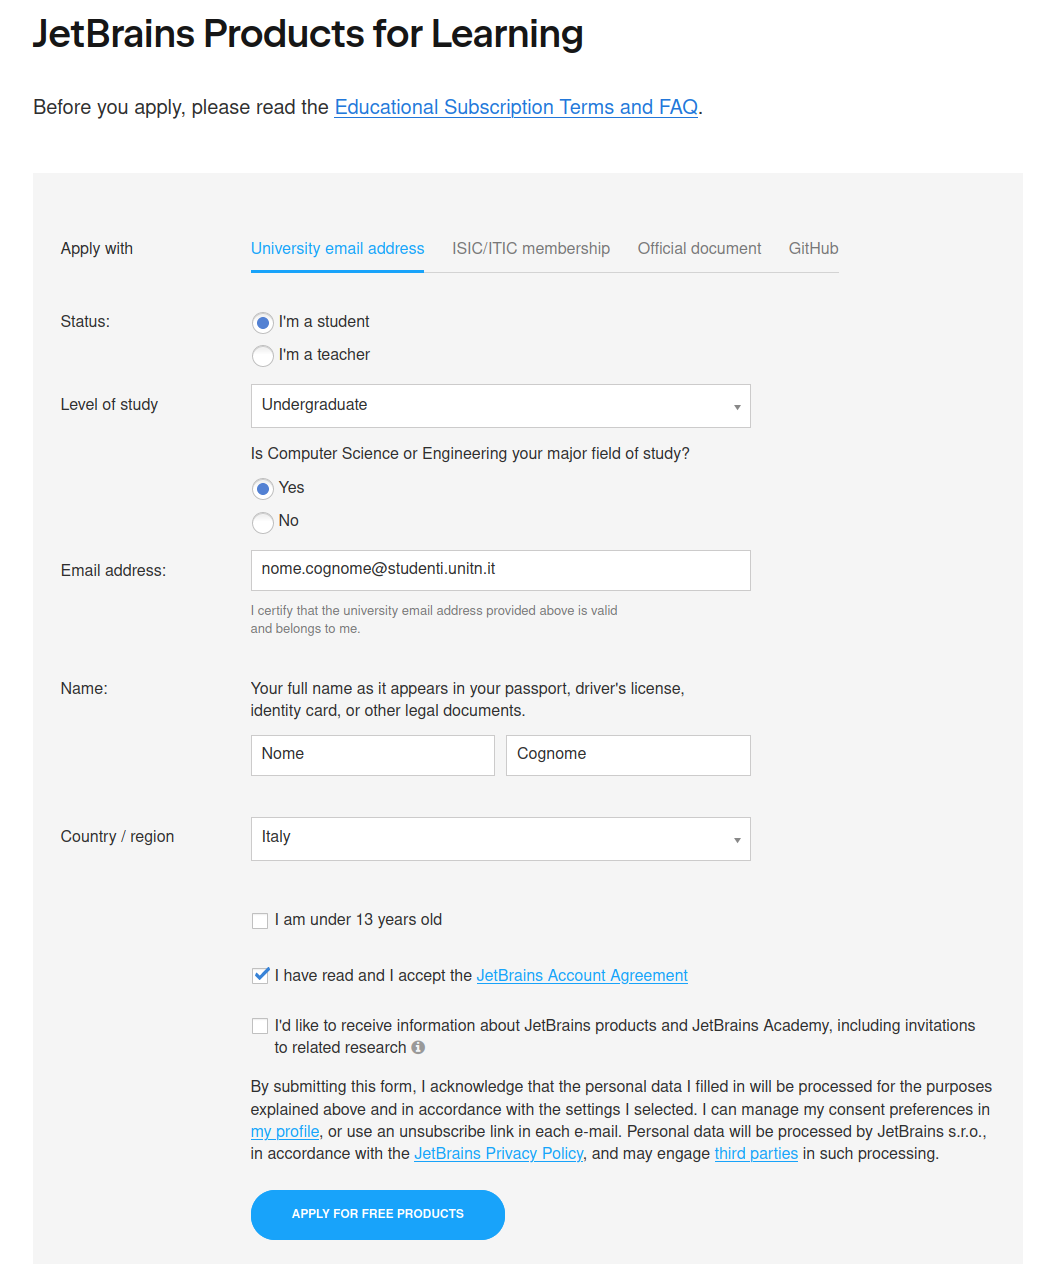
\includegraphics[width=1\textwidth]{form-studente-email.png}
                \caption{Form per la richiesta della licenza per studenti con email}
                \label{fig:Form per la richiesta della licenza per studenti con email}
            \end{figure}

            Una volta cliccato il bottone "Apply for free products" bisognerà completare il processo di certificazione aprendo il link ricevuto tramite email e completando 
            la creazione dell'account.
        
        \subsubsection{Certificato di iscrizione}
            Questa procedura richiede più passaggi, il primo dei quali è ottenere il certificato di iscrizione, andate su esse3, poi \textbf{Menù $\rightarrow$ Segreteria $\rightarrow$ My certificati} e in fine 
            cliccate su \textbf{Iscrizione con anni accademici (versione inglese)}. Scaricato il certificato tornate sulla pagina di JetBrains e selezionate apply with Official document, 
            compilate il form con i vostri dati, caricate il certificato e poi cliccate il bottone "Apply for free products".
            \begin{figure}[H]
                \centering
                \graphicspath{{src/capitoli/04/img/}}
                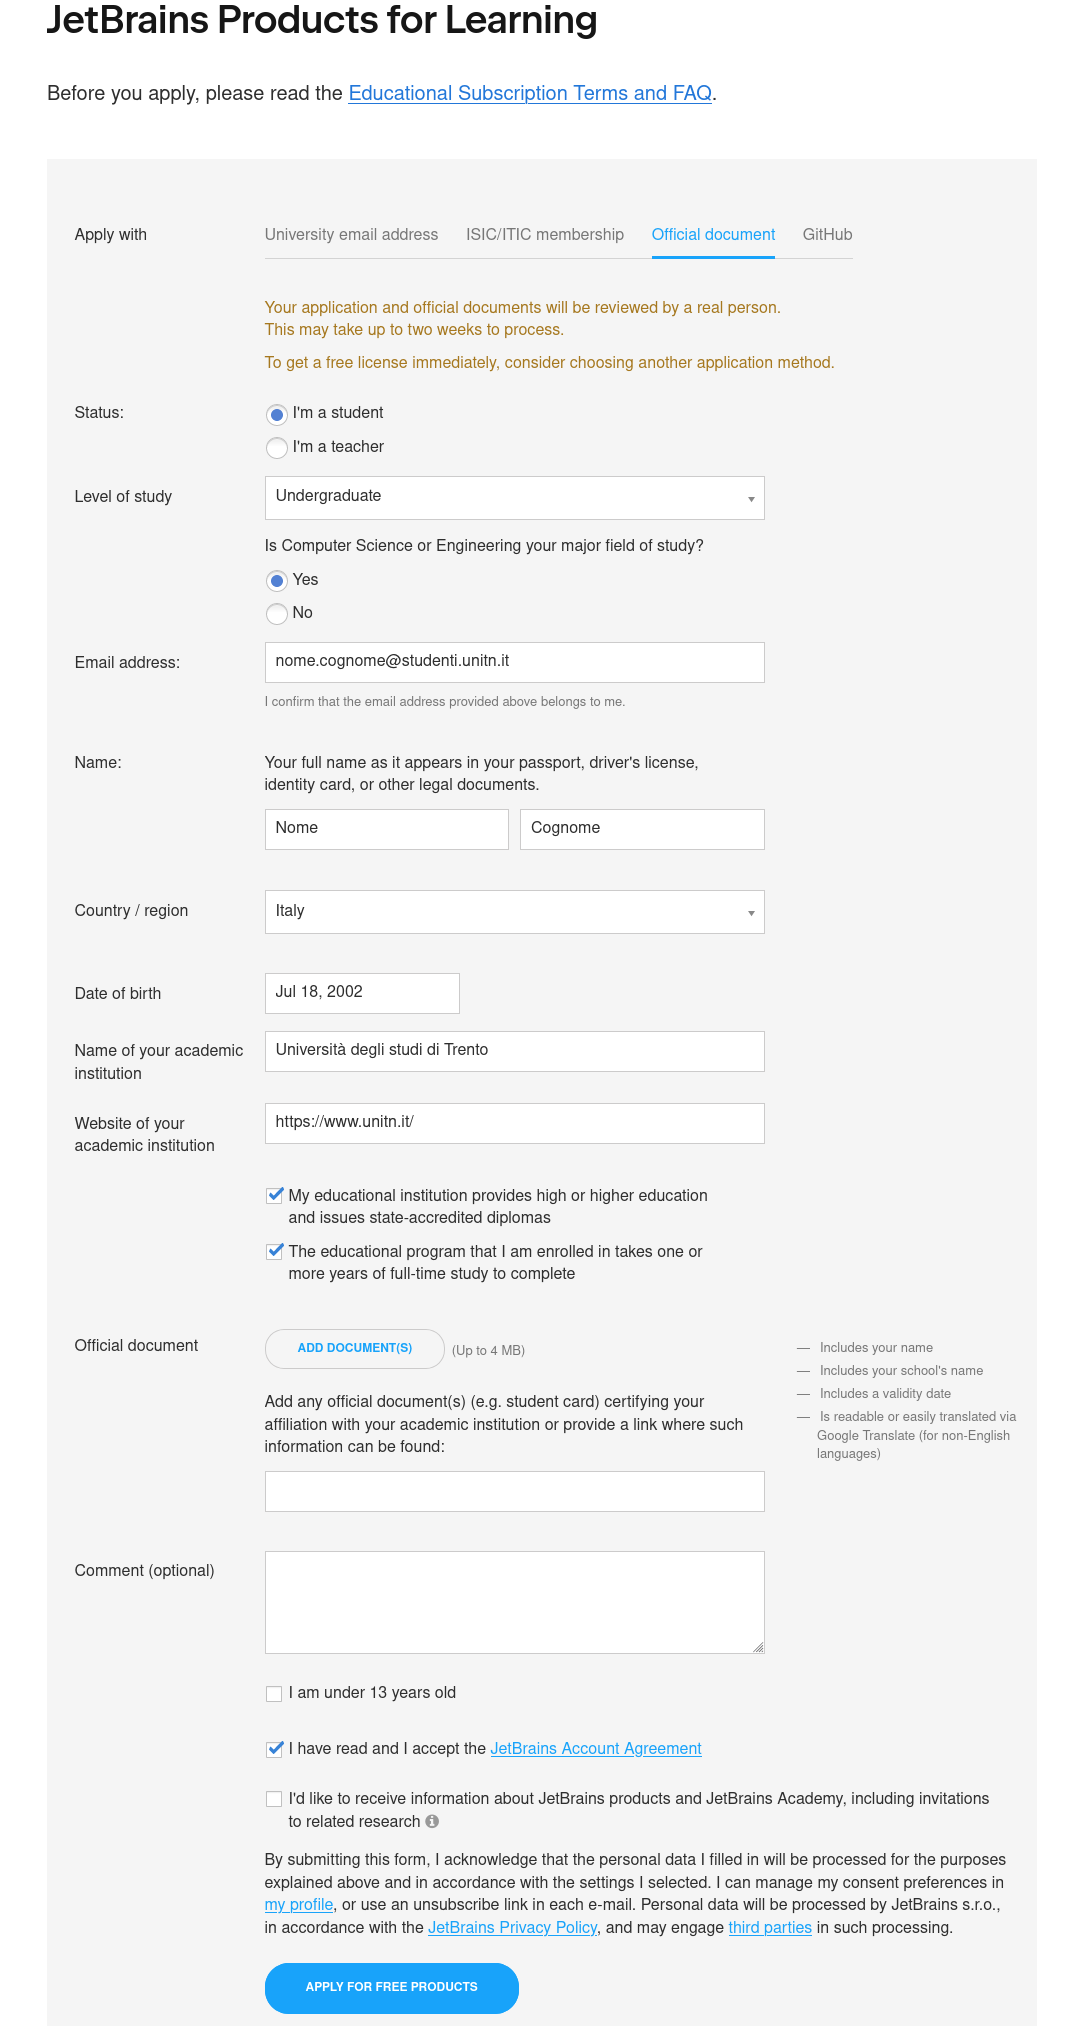
\includegraphics[width=0.7\textwidth]{form-studente-cert.png}
                \caption{Form per la richiesta della licenza per studenti con certificato}
                \label{fig:Form per la richiesta della licenza per studenti con certificato}
            \end{figure}
            Adesso dovete solo aspettare la mail di conferma per completare la creazione dell'account, solitamente richiede una settimana o più quindi abbiate pazienza.
    
    \subsection{Installare il ToolBox}
        Il modo più semplice per installare e mantenere aggiornati i prodotti JetBrains è utilizzare il ToolBox, un programma che 